\section{一些技巧}

\subsection{内存溢出及解决方案}
 
\paragraph{内存溢出}.所谓内存溢出,即  Out of memoery.

\begin{figure}[htbp]
\centering
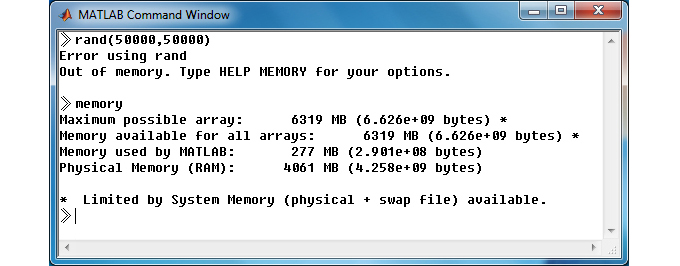
\includegraphics[width=9cm]{diagrams/memoryout.jpg}
\caption{内存溢出和内存查看}
\end{figure}

\vspace{-1.0cm}
\begin{lstlisting}[caption = 生成随机矩阵]
  matrix = rand(2e+5,2e+5);
\end{lstlisting}

\notation{逐渐增大或减小维数,这样可以查看设备能存储最大矩阵的维数.}


\paragraph{内存溢出解决}.简而言之,开源节流.\\
开源方法:
\begin{itemize*}
	\item 增加RAM.买个大点的内存条装上;
	\item 以“no java”方式启动MATLAB.
\end{itemize*}
节流方法:
\begin{itemize*}
	\item 数据本地存储.将数据存储到本地,需要时再导入;
	\item 使用已有的变量,即时删除临时变量(不再需要的变量);
	\item 以函数封装.将程序中某几部分的代码封装为 function 调用, function调用只输出最后需要的数据,其间的临时变量在每次调用完function之后都会自动删除.
\end{itemize*}



\subsection{大数据处理}
 提前给大数据分配内存. 过多小数据分配内存后形成的内存零碎化,这将可能使得.



\subsection{自定义函数使用help}
在MATLAB中可以用输入help加函数名来获得获悉使用方法及例子.我们期望对自己编写的函数也实现这样的功能,那么有两个关键点,一是参照MATLAB的内置函数注释格式写好注释(或者参照下面的示例),二是确保此函数路径已经添加.接下来就可以通过 \mcode{help myfunction} 这样的形式来查看了.

\vspace{-0.8cm}
\begin{lstlisting}[caption = 自定义帮助]
	function outputs = myfunction(inputs)
	%MYFUNCTION this function is bulabula...
	%   decrible your function here
	%   see also function1 function2

	%   Reversion: 22-Aug-2013
	%   2013/08/22  16:58:27
\end{lstlisting}



\subsection{获取图片}
\begin{itemize*}
	\item \mcode{print('-dpdf',pdf_name);}
	\item 直接设置导出
\end{itemize*}



\subsection{公式打印}
相关内容
\begin{itemize*}
	\item 图片上的公式
	\item 代码发布的公式
\end{itemize*}